A fase 2 do processo segue uma uma abordagem crowdsourcing para coletar as informações necessárias para gerar os conteúdos complementares que serão agregados ao vídeo. As atividades realizadas nesta fase são aquelas definidas no plano de ação.

\begin{figure}[ht]
\centering
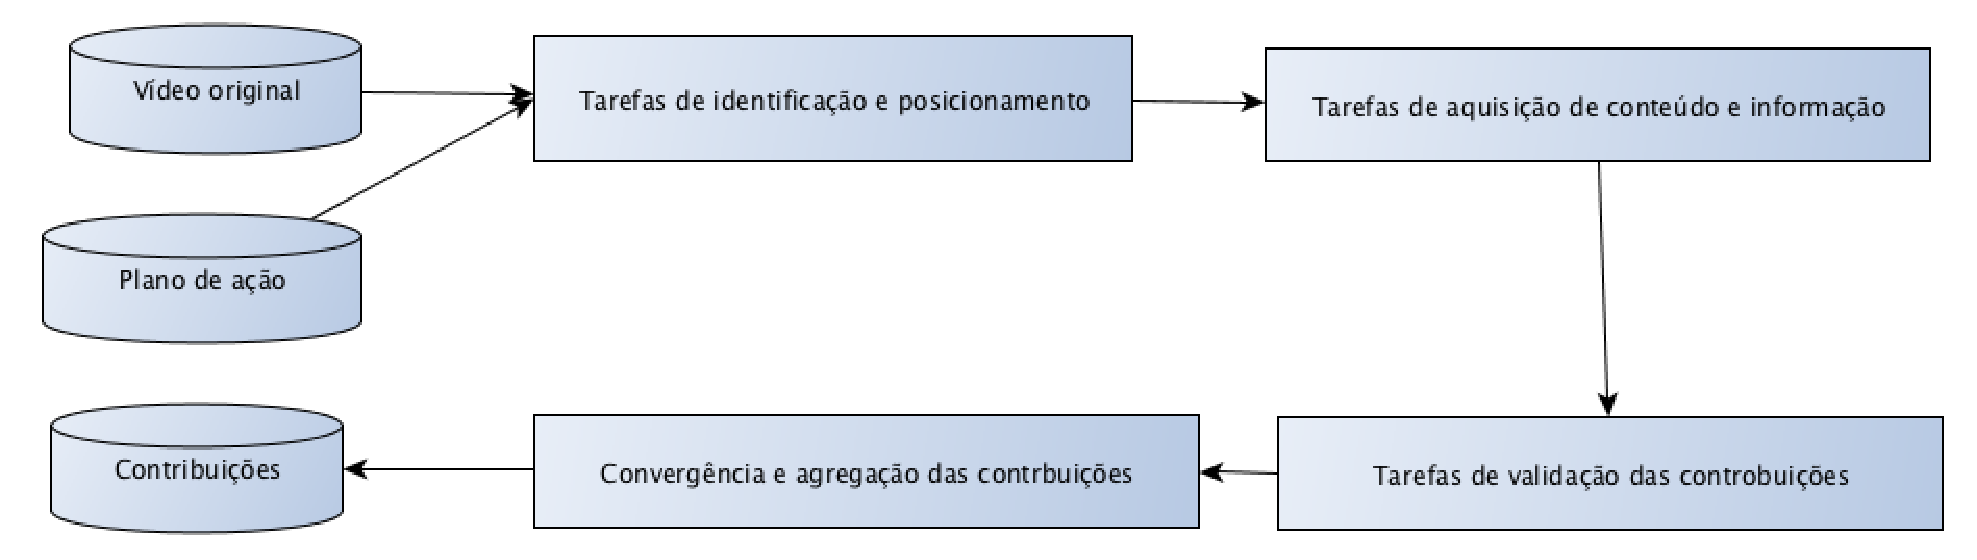
\includegraphics[width=.99\textwidth]{imagens/metodo/fase2_oa.eps}
\caption{Fase 2 do método}
\label{fig:metodo:fase2}
\end{figure}

Os três tipos de atividade, que foram modeladas como tarefas de anotação sobre o vídeo, são realizadas pelo Estudante. As tarefas são distribuídas entre eles de forma a coletar contribuições que possam cobrir todos os pontos identificados no plano de ação. Estes pontos dizem respeito aos tipos de ocorrência no vídeo sobre as quais se deseja coletar contribuições. De acordo com o plano de ação podem ser realizadas um, dois, ou os três tipos de tarefa. Entretanto, as atividades são realizadas na sequência em que aparecem na Figura~\ref{fig:metodo:fase2}. Desta forma é possível determinar onde estão as lacunas semânticas, coletar sugestões sobre como preenche-las, e avaliar quais delas mais satisfazem os estudantes.

Após se obter as contribuições necessárias para realizar a cobertura definida no plano de ação, são aplicadas técnicas de convergência e agregação para consolidar a base de contribuições que será utilizada para gerar o conteúdo complementar.

